%package list
\documentclass{article}
\usepackage[top=3cm, bottom=3cm, outer=3cm, inner=3cm]{geometry}
\usepackage{multicol}
\usepackage{graphicx}
\usepackage{url}
%\usepackage{cite}
\usepackage{hyperref}
\usepackage{array}
%\usepackage{multicol}
\newcolumntype{x}[1]{>{\centering\arraybackslash\hspace{0pt}}p{#1}}
\usepackage{natbib}
\usepackage{pdfpages}
\usepackage{multirow}
\usepackage[normalem]{ulem}
\useunder{\uline}{\ul}{}
\usepackage{svg}
\usepackage{xcolor}
\usepackage{listings}
\lstdefinestyle{ascii-tree}{
    literate={├}{|}1 {─}{--}1 {└}{+}1 
  }
\lstset{basicstyle=\ttfamily,
  showstringspaces=false,
  commentstyle=\color{red},
  keywordstyle=\color{blue}
}
%\usepackage{booktabs}
\usepackage{caption}
\usepackage{subcaption}
\usepackage{float}
\usepackage{array}

\newcolumntype{M}[1]{>{\centering\arraybackslash}m{#1}}
\newcolumntype{N}{@{}m{0pt}@{}}


%%%%%%%%%%%%%%%%%%%%%%%%%%%%%%%%%%%%%%%%%%%%%%%%%%%%%%%%%%%%%%%%%%%%%%%%%%%%
%%%%%%%%%%%%%%%%%%%%%%%%%%%%%%%%%%%%%%%%%%%%%%%%%%%%%%%%%%%%%%%%%%%%%%%%%%%%
\newcommand{\itemEmail}{jperez@unsa.edu.pe}
\newcommand{\itemStudent}{Juan Perez Luna}
\newcommand{\itemCourse}{Programación}
\newcommand{\itemCourseCode}{20231001}
\newcommand{\itemSemester}{I}
\newcommand{\itemUniversity}{Universidad Nacional de San Agustín de Arequipa}
\newcommand{\itemFaculty}{Facultad de Ingeniería de Producción y Servicios}
\newcommand{\itemDepartment}{Departamento Académico de Ingeniería de Sistemas e Informática}
\newcommand{\itemSchool}{Escuela Profesional de Ingeniería de Sistemas}
\newcommand{\itemAcademic}{2023 - A}
\newcommand{\itemInput}{Del 10 Abril 2023}
\newcommand{\itemOutput}{Al 17 Abril 2023}
\newcommand{\itemPracticeNumber}{01}
\newcommand{\itemTheme}{Git y GitHub}
%%%%%%%%%%%%%%%%%%%%%%%%%%%%%%%%%%%%%%%%%%%%%%%%%%%%%%%%%%%%%%%%%%%%%%%%%%%%
%%%%%%%%%%%%%%%%%%%%%%%%%%%%%%%%%%%%%%%%%%%%%%%%%%%%%%%%%%%%%%%%%%%%%%%%%%%%

\usepackage[english,spanish]{babel}
\usepackage[utf8]{inputenc}
\AtBeginDocument{\selectlanguage{spanish}}
\renewcommand{\figurename}{Figura}
\renewcommand{\refname}{Referencias}
\renewcommand{\tablename}{Tabla} %esto no funciona cuando se usa babel
\AtBeginDocument{%
	\renewcommand\tablename{Tabla}
}

\usepackage{fancyhdr}
\pagestyle{fancy}
\fancyhf{}
\setlength{\headheight}{30pt}
\renewcommand{\headrulewidth}{1pt}
\renewcommand{\footrulewidth}{1pt}
\fancyhead[L]{\raisebox{-0.2\height}{
\includegraphics[width=3cm]{img/logo_episunsa.png}}}
\fancyhead[C]{\fontsize{7}{7}\selectfont	\itemUniversity \\ \itemFaculty \\ \itemDepartment \\ \itemSchool \\ \textbf{\itemCourse}}
\fancyhead[R]{\raisebox{-0.2\height}{
\includegraphics[width=1.2cm]{img/logo_abet}}}
\fancyfoot[L]{Estudiante Juan Perez Perez}
\fancyfoot[C]{\itemCourse}
\fancyfoot[R]{Página \thepage}

% para el codigo fuente
\usepackage{listings}
\usepackage{color, colortbl}
\definecolor{dkgreen}{rgb}{0,0.6,0}
\definecolor{gray}{rgb}{0.5,0.5,0.5}
\definecolor{mauve}{rgb}{0.58,0,0.82}
\definecolor{codebackground}{rgb}{0.95, 0.95, 0.92}
\definecolor{tablebackground}{rgb}{0.8, 0, 0}

\lstset{frame=tb,
	language=bash,
	aboveskip=3mm,
	belowskip=3mm,
	showstringspaces=false,
	columns=flexible,
	basicstyle={\small\ttfamily},
	numbers=none,
	numberstyle=\tiny\color{gray},
	keywordstyle=\color{blue},
	commentstyle=\color{dkgreen},
	stringstyle=\color{mauve},
	breaklines=true,
	breakatwhitespace=true,
	tabsize=3,
	backgroundcolor= \color{codebackground},
}

\begin{document}
	
	\vspace*{10px}
	
	\section{Tipo de Sistema}
		\begin{itemize}		
			\item 
		\end{itemize}
			
	\section{Requisitos del sistema}
		\begin{itemize}
			\item 
		\end{itemize}
		
	\section{Modelo de datos}
		\begin{itemize}
			\item 
		\end{itemize}
		
	\section{Diccionario de datos}
	\begin{itemize}
		\item \textbf{Categoria:}
	
	Campos: nombre, descripcion
	Descripción: Este modelo almacena información sobre las categorías de productos disponibles en la cafetería. Cada categoría tiene un nombre y una descripción.
	\begin{figure}[h!]
		\centering
		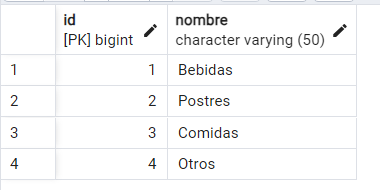
\includegraphics[width=1\linewidth]{img/tcategoria}
		\caption{Tabla de categoria}
		\label{fig:tcategoria}
	\end{figure}
	
		\item \textbf{Producto:}
	
	Campos: categoria, nombre, descripcion, precio, imagen
	Descripción: El modelo de Producto guarda detalles sobre los productos ofrecidos en la cafetería. Cada producto está asociado a una categoría y tiene un nombre, descripción, precio y una imagen.
	\begin{figure}[h!]
		\centering
		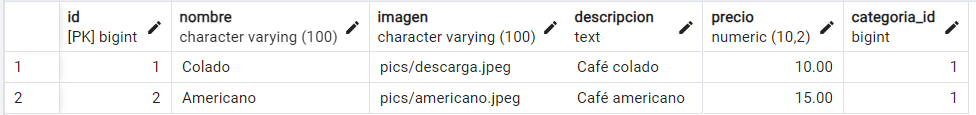
\includegraphics[width=1\linewidth]{img/tproducto}
		\caption{Tabla producto}
		\label{fig:tproducto}
	\end{figure}
	
		\item \textbf{Cliente:}
	
	Campos: nombre, apellido, correo, telefono
	Descripción: El modelo de Cliente almacena información de los clientes que visitan la cafetería. Incluye el nombre, apellido, correo electrónico y número de teléfono de los clientes.
	\begin{figure}[h!]
		\centering
		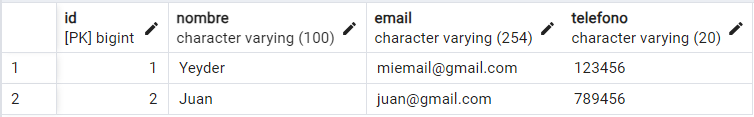
\includegraphics[width=1\linewidth]{img/tcliente}
		\caption{tabla de cliente}
		\label{fig:tcliente}
	\end{figure}
	
		\item \textbf{Pedido:}
		
		Campos: cliente, producto, fecha-pedido, estado
		Descripción: El modelo de Pedido registra los pedidos realizados por los clientes. Cada pedido tiene un cliente asociado, un producto solicitado, la fecha del pedido y su estado (pendiente, entregado, etc.).
		\begin{figure}[h!]
			\centering
			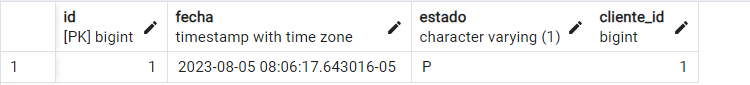
\includegraphics[width=1\linewidth]{img/tpedido}
			\caption{Tabla pedido}
			\label{fig:tpedido}
		\end{figure}
		
	
		\item \textbf{itemPedido:}
	
	Campos: pedido, cantidad
	Descripción: El modelo de DetallePedido guarda información sobre los productos y las cantidades asociadas a un pedido específico. Cada detalle de pedido está vinculado a un pedido y registra la cantidad de un producto solicitado.
	\begin{figure}[h!]
		\centering
		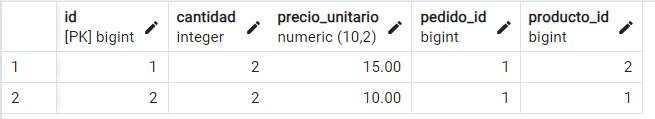
\includegraphics[width=1\linewidth]{img/titempedido}
		\caption{Tabla itemPedido}
		\label{fig:titempedido}
	\end{figure}
	
		\item \textbf{Carrito:}
		
	Campos: cliente
	Descripción: El modelo "Carrito" representa el carrito de compras de un cliente. Está asociado a un cliente específico y actúa como un contenedor temporal para los productos que el cliente planea comprar.
	\begin{figure}[h!]
		\centering
		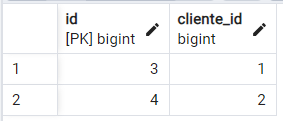
\includegraphics[width=1\linewidth]{img/tcarrito}
		\caption{Tabla carrito}
		\label{fig:tcarrito}
	\end{figure}
	
		\item \textbf{ItemCarrito:}
		
	Campos: carrito, producto, cantidad
	Descripción: El modelo "ItemCarrito" registra los productos y las cantidades agregadas al carrito de compras de un cliente. Cada elemento del carrito está vinculado a un carrito, un producto específico y la cantidad deseada.
	\begin{figure}[h!]
		\centering
		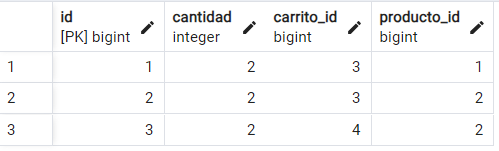
\includegraphics[width=1\linewidth]{img/titemcarrito}
		\caption{Tabla itemCarrito}
		\label{fig:titemcarrito}
	\end{figure}
	
	\end{itemize}
		
	\section{Diagrama Entidad-Relación (ERD)}
	En esta sección se mostrará los modelos creados con sus respectivos campos en el proyecto y la relación entre cada uno de ellos.
	
	Inicialmente se mostrará cada uno de las tablas y sus relaciones, para una mejor comprensión, las tablas genteradas son: categoria, producto, cliente, carrito, pedido, itemcarrito e itempedido.
	
	\subsection{modelo categoria}
	Consta de un campo "nombre" y tiene una relación de uno a muchos con el modelo producto, esto porque una categoría (bebidas, postres y entre otros) pueden tener muchos productos.
	\begin{figure}[h!]
		\centering
		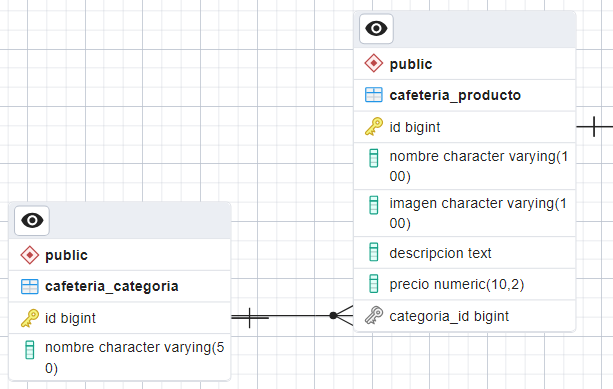
\includegraphics[width=1\linewidth]{img/modCategoria}
		\caption{Figura de del modelo categoria y sus relaciones}
		\label{fig:modcategoria}
	\end{figure}
	
	\subsection{modelo producto}
	Consta de de campos como nombre, imagen, descripción, precio y tiene una relación de mushos a uno con categoría, como se explicó anteriormente, y también tiene una relación de uno a muchos con itemcarrito e itempedido (ambos).
	\begin{figure}[h!]
		\centering
		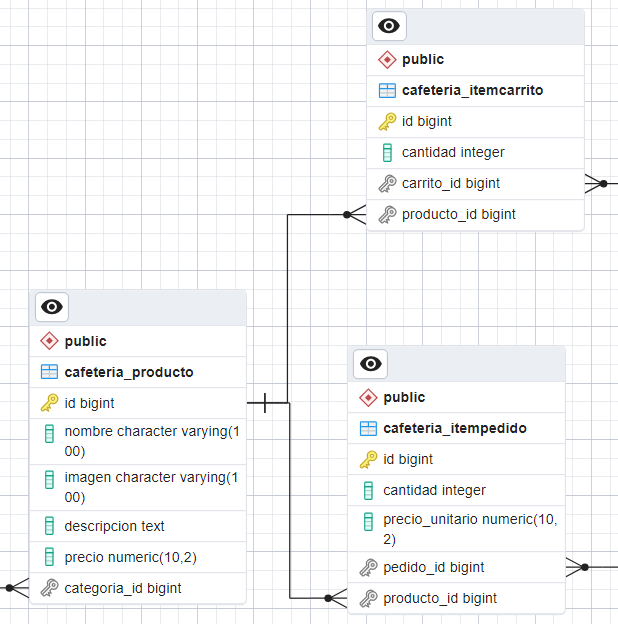
\includegraphics[width=1\linewidth]{img/modProducto}
		\caption{Figura de del modelo producto y sus relaciones}
		\label{fig:modproducto}
	\end{figure}
	\newpage
	\subsection{modelo cliente, carrito, pedido}
	El modelo cliente consta de campos como nombre, email y telefono, y tiene  una relación de uno a muchos con carrito e edido (ambos). A su vez el modelo carrito tiene una relación de uno a muchos con el modelo itemcarrito, puede tene muchos itme carrito que su su vez guardan productos. Por otro lado, el modelo pedido también tiene una relación de uno a muchos con el modelo itempedido, y esta guarda a productos.
	\begin{figure}[h!]
		\centering
		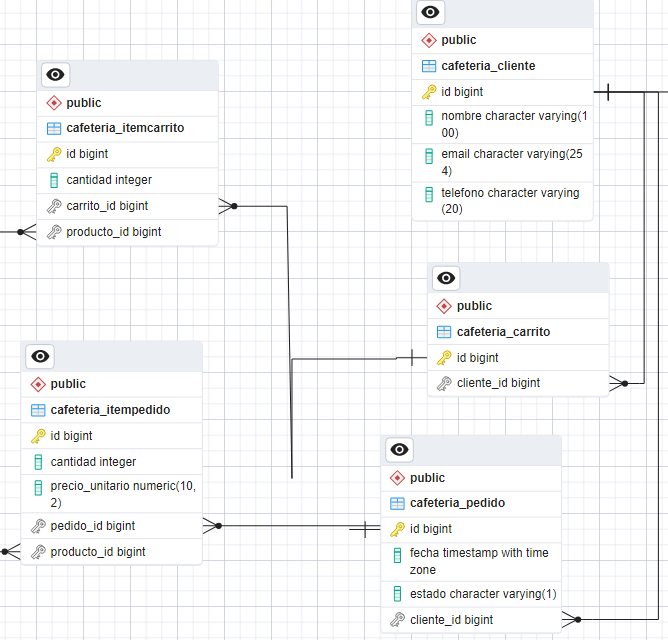
\includegraphics[width=1\linewidth]{img/modClienteotros}
		\caption{Figura de del modelo cliente, carrito y pedido con sus respactivas relaciones}
		\label{fig:modclienteotros}
	\end{figure}
	\newpage
	\subsection{modelo cliente, carrito, pedido}
	Antes de ver estos modelos, debemos tener en cuenta que estos modelos sirven como enlace a producto con carrito y pedido, esta relación inicialmente se consideraba de muchos a muchos, sin embargo, Django genera otra tabla por defecto con relación de uno a muchos. Estas tablas cumplen la misma funcionalidad y tienen algunos campos más.
	\begin{figure}[h!]
		\centering
		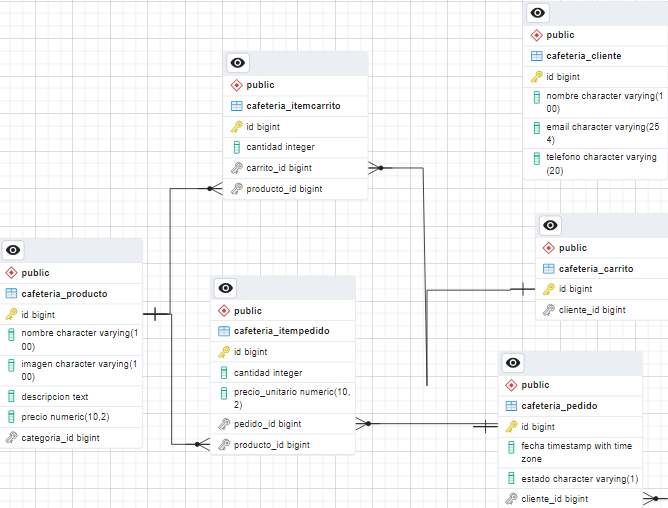
\includegraphics[width=1\linewidth]{img/modItems}
		\caption{Figura de del modelo itemcarrito e itempedido con sus respactivas relaciones}
		\label{fig:moditems}
	\end{figure}
	\newpage
	\subsection{modelo ERD}
	Ahora se mostrará la tabla con los modelos completos y sus respectivas relaciones.
	\begin{figure}[h!]
		\centering
		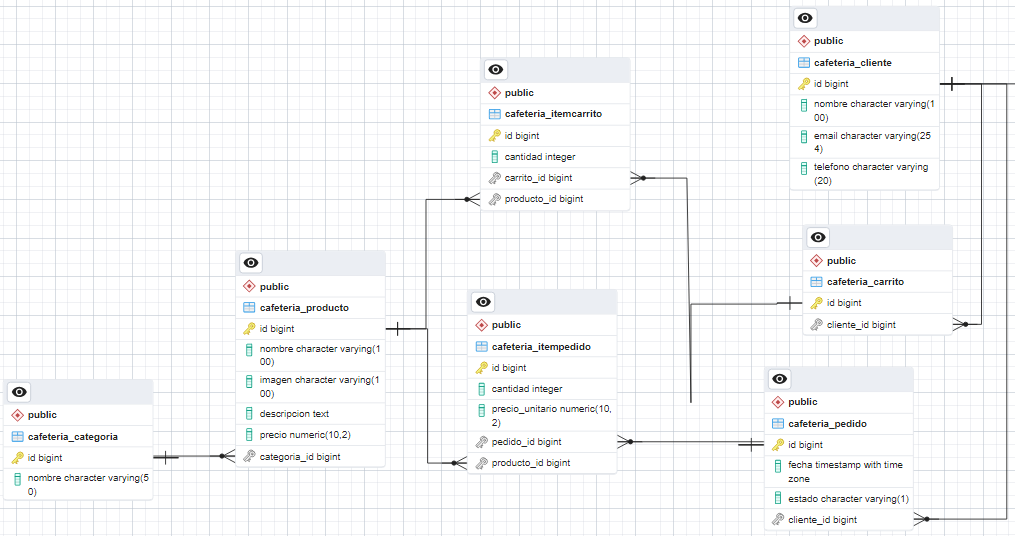
\includegraphics[width=1\linewidth]{img/DER}
		\caption{Se puede visualizar el Diagrama Entidad Relación completo, con los 7 modelos creados en código}
		\label{fig:der}
	\end{figure}	
	
	\section{Administración con Django}
		
		
	
	\section{CRUD - Core Business - Clientes finales}
	\section{Investigación: Email, Upload}
	
	\section{REFERENCIAS}
	
	\begin{itemize}			
		\item \url{https://www.w3schools.com/java/default.asp}
		\item \url{https://www.geeksforgeeks.org/insertion-sort/}
	\end{itemize}	
	
%\clearpage
%\bibliographystyle{apalike}
%\bibliographystyle{IEEEtranN}
%\bibliography{bibliography}
			
\end{document}